\documentclass{article}
\usepackage[utf8]{inputenc}
\usepackage{amsmath}
\usepackage{amssymb}
\usepackage{mathtools}
\usepackage{graphicx}

\graphicspath{{Images/}}

\setlength{\oddsidemargin}{0in}
\setlength{\textwidth}{6.5in}
\setlength{\topmargin}{-.55in}
\setlength{\textheight}{9in}
\pagestyle{empty}


\title{Solid State Physics Midterm 1 Take Home}
\author{Michael Nameika}
\date{October 2022}

\begin{document}

\maketitle

\section*{Problem 4} Measurements for copper gives the mean-squared displacement of the atoms from their average positions as 0.021 $\text{\AA}^2$ at 293 K, and 0.096 $\text{\AA}^2$ at 1273 K. 
Cu has fcc structure with $a = 3.615 \text{\AA}$ and we will neglect the fact that the lattice constant changes with temperature. 
Calculate the ratios of intensities at the two temperatures of (a) the lowest angle and (b) highest-angle reflections that can be measured with Mo$\text{K}_{\alpha1}$ radiation ($\lambda = 0.070926 \text{nm}$)? 
How much would these ratios change if you would use Cu radiation ($\lambda = 0.15406 \text{nm}$)?
Can you detect XRD peaks at the highest angles for both types of radiation?
\newline\newline
(a) To begin, recall that intensity of scattered radiation is approximately given by
\[I \approx \exp{\left(-\frac{1}{2}\frac{\langle u^2 \rangle \langle G^2 \rangle}{3}\right)}\]
Also recall that $|G| = \frac{2\pi}{d_{hkl}}$. So $\langle G^2 \rangle \approx \frac{4\pi^2}{d^2_{hkl}}$. And $d_{hkl}$ is given by $d_{hkl} = \frac{a}{\sqrt{h^2 + k^2 + l^2}}$. Now, recall that the lowest reflection angle for an fcc lattice occurs for the (111) plane. That is,
\begin{align*}
    d_{111} &= \frac{a}{\sqrt{3}} \\
    &= \frac{3.615 \text{\AA}}{\sqrt{3}} \\
    &\approx 2.087 \text{\AA} \\
\end{align*}
so
\begin{align*}
    \langle G^2 \rangle &= \frac{4\pi^2}{2.087^2} \text{\AA}^{-2} \\
    &\approx 9.064 \text{\AA}^{-2} \\
\end{align*}
Now, for 293 K, our $\langle u^2 \rangle = 0.021 \text{\AA}^2$ and so our intensity for the lowest angle reflection at 293 K is given by
\begin{align*}
    I_{293K} &= \exp{\left(-\frac{1}{2}\frac{(0.021)(9.064)}{3}\right)} \\
    &\approx 0.9688 \\
\end{align*}
And now, at 1273 K, $\langle u^2 \rangle = 0.096 \text{\AA}^2$ and so our intensity for the lowest angle reflection at 1273 K is given by
\begin{align*}
    I_{1273K} &= \exp{\left(-\frac{1}{2}\frac{(0.096)(9.064)}{3}\right)} \\
    &\approx 0.8650 \\
\end{align*}
And the ratio between the two:
\begin{align*}
    \frac{I_{293K}}{I_{1273K}} &= \frac{0.9688}{0.8650} \\
    &\approx 1.12 \\
\end{align*}
So the intensity of the lowest angle reflection is only approximately 12\% stronger at 293K. 
\newline
(b) Now for the highest angle reflection, we must calculate what the highest possible reflection allowed by Mo$\text{K}_{\alpha 1}$ radiation. Well, from Bragg's law (assuming $n = 1$), we have
\[\sin{(\theta)} = \frac{\lambda}{2d}\]
Now, since $\sin{(\theta)}$ is bounded between $\pm 1$, we require $\frac{\lambda}{2d} \leq 1$. then substituting, we find
\begin{align*}
    \sqrt{h^2 + k^2 + l^2} &\leq \frac{2a}{\lambda} \\
\end{align*}
and 
\begin{align*}
    \frac{2a}{\lambda} &= \frac{2(3.615 \text{\AA})}{0.70926 \text{\AA}} \\
    &\approx 10.194 \\
\end{align*}
then
\begin{align*}
    h^2 + k^2 + l^2 &\leq (10.194)^2 \\
    &\approx 104 \\
\end{align*}
So we require $h^2 + k^2 + l^2 \leq 104$. Notice that the plane (862) satisfies this, and is an allowed reflection plane for an fcc lattice. Now, let us calculate $d_{862}$:
\begin{align*}
    d_{862} &= \frac{a}{\sqrt{104}} \\
    &= \frac{3.615 \text{\AA}}{\sqrt{104}} \\
    &\approx .3545 \text{\AA}\\
\end{align*}
Then as in part (a), 
\begin{align*}
    \langle G^2 \rangle &= \frac{4 \pi^2}{d^2} \\
    &= \frac{4 \pi^2}{.3545^2} \text{\AA}^{-2} \\
    &\approx 314.14 \text{\AA}^{-2} \\
\end{align*}
Now, our scattered intensity at 293 K is
\begin{align*}
    I_{293 K} &= \exp{\left(-\frac{1}{2}\frac{\langle u^2 \rangle \langle G^2 \rangle}{3}\right)}\\
    &= \exp{\left(-\frac{1}{2}\frac{(0.021)(314.14)}{3}\right)} \\
    &\approx 0.333 \\
\end{align*}
And the scattered intensity at 1273 K is
\begin{align*}
    I_{1273 K} &= \exp{\left(-\frac{1}{2} \frac{\langle u^2 \rangle \langle G^2 \rangle}{3}\right)} \\
    &= \exp{\left(-\frac{1}{2}\frac{(0.096)(314.14)}{3}\right)} \\
    &\approx 6.563\times 10^{-3} \\
\end{align*}
And finally, the ratio between the two:
\begin{align*}
    \frac{I_{293 K}}{I_{1273 K}} &= \frac{0.333}{6.3563 \times 10^{-3}} \\
    &\approx 52.39 \\
\end{align*}
So the intensity of the lowest angle reflection to the greatest angle reflection for Mo $\text{K}_{\alpha 1}$ radiation is 52.39 times stronger.
\newline
Now suppose we use Cu radiation ($\lambda = 1.5406 \text{\AA}$). Notice that the lowest angle reflection and intensities will stay the same, since it did not depend on $\lambda$. However, the highest angle reflection will change. Similar to the work above, we require $\frac{\lambda}{2d} \leq 1$. Then
\begin{align*}
    \sqrt{h^2 + k^2 + l^2} &\leq \frac{2a}{\lambda} \\
    \frac{2a}{\lambda} &= \frac{2(3.615 \text{\AA})}{1.5406\text{\AA}} \\
    &\approx 4.693 \\
\end{align*}
so 
\begin{align*}
    h^2 + k^2 + l^2 &\leq (4.693)^2 \\
    &\approx 22 \\
\end{align*}
Recall that the allowed indices for reflection of an fcc lattice must be equal to 0 or 3 mod 4. However, $22 = 2 \mod{4}$, so this is not an allowed reflection for copper. The next allowed plane that satisfies the above inequality is when $h^2 + k^2 + l^2 = 20$, which corresponds to the plane (422).
Then 
\begin{align*}
    d_{442} &= \frac{3.615 \text{\AA}}{\sqrt{20}} \\
    &= .8083 \text{\AA} \\
\end{align*}
so
\begin{align*}
    |G|^2 &= \frac{4\pi^2}{0.8083^2} \text{\AA}^{-2} \\
    &\approx 60.425 \text{\AA}^{-2} \\
\end{align*}
Now let us calculate the intensities of reflection on this plane for 293 K and 1273 K:
\begin{align*}
    I_{293 K} &= \exp{\left(-\frac{1}{2}\frac{0.021(60.425)}{3}\right)} \\
    &\approx 0.8049 \\
\end{align*}
and
\begin{align*}
    I_{1273 K} &= \exp{\left(-\frac{1}{2}\frac{0.096(60.425)}{3}\right)} \\
    &\approx 0.3803 \\
\end{align*}
and the ratio between them:
\begin{align*}
    \frac{I_{293 K}}{I_{1273 K}} &= \frac{0.8083}{0.3803} \\
    &\approx 2.125 \\
\end{align*}
So for $\lambda = 1.5406 \text{\AA}$, the intensity of reflection at the greatest angle is a little over twice as intense at 293 K than it is at 1273 K.
\newline

For $\lambda = 1.5406 \text{\AA}$, we can definitely detect the peaks of XRD for the greatest angle of reflection (it's only different by a factor of 2!). For $\lambda = 0.70926 \text{\AA}$, and we can still expect to detect the peak at the highest angle of reflection. Looking back at homework 3, we had detectable peaks that were over 1/100th the intensity of the major peaks.

\section*{Problem 5} Perovskite compound, $\text{KZnF}_3$, has a cubic structure and lattice constant of $4.054 \text{\AA}$. Imagine that I will soon send you X-ray data from the powder sample measured in the $\Theta - 2\Theta$ experiment. You also know that in the experiment I used Cu radiation ($\lambda = 1.5406 \text{\AA}$). Determine the structural factor, $\text{S}_{\text{G}}$, for this compound. Assume that a single F atom scatters X-ray with amplitude f, K with amplitude 2f, and Zn with amplitude 3f. (These assumptions must be almost right since Z numbers are 9, 19, and 30 for these elements).
\newline\newline
To begin, notice we have one Zn atom, one K atom, and 3 F atoms per cell. we will find the structural factor of Perovskite. Recall the formula for the structural factor for a crystal is given by the following:
\[S_g = \sum_j f_je^{-2i\pi(hx_j + ky_j + lz_j)}\]
Using this, we find
\begin{align*}
    S_{g,Perov} &= f_1e^{-i\pi(0)} + f_2e^{-i\pi(h + l)} + f_3e^{-i\pi(k + l)} + f_4e^{-i\pi(h + k)} + f_5e^{-i\pi(h + k + l)} \\
    &= f + 2fe^{-i\pi(h+l)} + 2fe^{-i\pi(k+l)} + 2fe^{-i\pi(h + k)} + 3fe^{-i\pi(h + k + l)} \\
    &= f(1 + 2e^{-i\pi(h + l)} + 2e^{-i\pi(k+l)} + 2e^{-i\pi(h + k)} + 3e^{-i\pi(h + k + l)}) \\
 \end{align*}
\begin{enumerate}
    \item[a)] Determine the positions of the diffraction peaks and their intensities. In order to make my life easier, for the most intense peak assign intensity = 100, while for background (no peak) value 0. Prepare a table which will consist of 4 columns with hkl, $2\Theta$, $\text{S}_{\text{G}}$, and intensity values (in this part of the problem let's neglect the fact that with increasing hkl values the intensity of the peaks will decay as we have shown in class due to changes in an atomic factor). Document your analysis! Plot calculated intensity vs. $2\Theta$ (up to 120 deg.). Your plot will not be realistic but it will be a good start to determine a diffraction pattern of this compound.
    \newline
    
    To find the peak positions of the diffraction peaks, we must find when $S_{g, Perov}$ is maximized. Well, begin by noticing if all $h,k,l \in 2\mathbb{Z}$, then each exponential in $S_{g, Perov}$ is maximized (equal to one) and so our structure factor will equal 10$f$. Similarly, if each $h,k,l$ is odd, we notice the exponentials with terms of only two of $h,k,l$ will be maximized, and $e^{-i\pi(h + k + l)} = -1$, so our structure factor in this case will come to 4. Now, consider the case where one of $h,k,l$ is odd and two are even. Without loss of generality, let $h = 2n + 1$, $k = 2m$, $l = 2r$, for some $m,n,r$. Then
    \begin{align*}
        S_{g, Perov} &= f(1 + 2e^{-i\pi(2n + 1)} + 2e^{-i\pi(2m)} + 2e^{-i\pi(2r)} + 3e^{-i\pi(2n + 1 + 2m + 2r)}) \\
        &= f(1 - 2 + 2 + 2 - 3) \\
        &= 0 \\
    \end{align*}
    Now consider the case where one of $h,k,l$ is even and two are odd. Without loss of generality, let $h = 2n$, $k = 2m + 1$, $l = 2r + 1$, for some $m,n,r \in \mathbb{Z}$. Then
    \begin{align*}
        S_{g, Perov} &= f(1 + 2e^{-i\pi(2n)} + 2e^{-i\pi(2m + 1)} + 2e^{-i\pi(2r + 1)} + 3e^{-i\pi(2n + 2m + 1 + 2r + 1)} \\
        &= f(1 + 2 - 2 - 2 + 3) \\
        &= 2 \\
    \end{align*}
    So we have (without loss of generality)
    \[S_{g, Perov} = \begin{cases}
        10f & h,k,l \:\: \text{even} \\
        4f & h,k,l \:\: \text{odd} \\
        2f & h \:\: \text{even};\:\: k,l \:\: \text{odd} \\
        0 & h,k \:\: \text{even}; \:\: l \:\: \text{odd} \\
    \end{cases}\]
    
    Now, we wish to find the allowed reflections for $2\Theta$ up to 120 degrees. To do so, from Bragg's law, we have
    \[\sin{(\theta)} = \frac{\lambda\sqrt{h^2 + k^2 + l^2}}{2a}\]
    We need to find all planes where up 120 degrees, so we must bound the right hand side of the above equation by $\sqrt{3}/2$. Doing so leads to the following expression:
    \begin{align*}
        h^2 + k^2 + l^2 &= \frac{3a^2}{\lambda^2} \\
        &= \frac{3(4.054 \text{\AA})^2}{(1.5406 \text{\AA})^2} \\
        &\approx 20 \\
    \end{align*}
    So we require $h^2 + k^2 + l^2 \leq 20$. Then the Miller indices that satisfy this along with the restrictions on $S_{g, Perov}$, we have the allowed planes are given by
    \begin{center}
    \begin{tabular}{c c}
         (110) & (111) \\
         (200) & (211) \\
         (222) & (310) \\
         (311) & (321) \\
         (331)\\
    \end{tabular}
    \end{center}
    Now we must compute the $\Theta$ values associated with each of these indices. From Bragg's law,
    \[\theta = \arcsin{\left(\frac{\lambda\sqrt{h^2 + k^2 + l^2}}{2a}\right)}\]
    Now calculating all the $\Theta$ values for the Miller indices, along with the structural factor and intensity values, we find the following table:
    \begin{center}
        \begin{tabular}{c|c|c|c|c}
             $i$ & $(hkl)$ & $2\Theta$ & $S_g$ & intensity\\
             \hline
             1 & (110) & $31.18^{\circ}$ & $2f$ & 20 \\
             2 & (111) & $38.43^{\circ}$ & $4f$ & 40 \\
             3 & (200) & $44.67^{\circ}$ & $10f$ & 100 \\
             4 & (211) & $55.48^{\circ}$ & $2f$ & 20 \\
             5 & (222) & $82.33^{\circ}$ & $10f$ & 100 \\
             6 & (310) & $73.86^{\circ}$ & $2f$ & 20 \\
             7 & (311) & $78.13^{\circ}$ & $4f$ & 40 \\
             8 & (321) & $90.62^{\circ}$ & $2f$ & 20 \\
        \end{tabular}
    \end{center}
    Plotting these using Gaussians (I used $I\exp{(-(x-2\Theta)^2/0.15^2)}$ for each peak) to model the diffraction peaks in MATLAB, we find the following:
    \begin{center}
        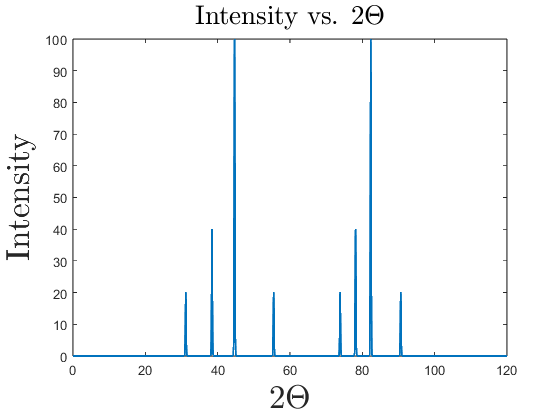
\includegraphics[scale = 0.6]{Intensity.png}
    \end{center}
    
    
    \item[b)] In class I have shown you that an atomic factor is not a constant as you can see from the figure below. Use this data to generate a plot of the more realistic diffraction pattern of $\text{KZnF}_3$ sample. Again, assign to the most intensive peak value of 100. Document your analysis! Prepare a new table with "corrected peak intensities." Plot calculated intensity vs $2\Theta$ (up to 120 deg.). It will be fun to compare your results with the realistic diffraction pattern which I will generate.
    \newline
    Let us begin by calculating the values for $\frac{\sin{(\theta)}}{\lambda}$ for our values of $\theta$:
    \begin{center}
    \begin{tabular}{c|c}
        $2\Theta$ & $\frac{\sin{(\theta)}}{\lambda} [\AA]^{-1}$ \\
        \hline 
        $31.18^{\circ}$ & 0.1722 \\
        $38.45^{\circ}$ & 0.2109 \\
        $44.67^{\circ}$ & 0.2435 \\
        $55.48^{\circ}$ & 0.2983 \\
        $73.86^{\circ}$ & 0.3851 \\
        $78.13^{\circ}$ & 0.4039 \\
        $82.33^{\circ}$ & 0.4218 \\
        $90.62^{\circ}$ & 0.4556 \\
    \end{tabular}
    \end{center}
    
    Using the given plot to approximate how the atomic factor (using the curve for Ne), we find that the atomic factor decreases by (roughly) the following factors:
    \begin{center}
        \begin{tabular}{c|c}
            $\frac{\sin{(\theta)}}{\lambda} [\AA]^{-1}$ & Approx. Weight \\
            \hline
            0.1722 & 0.85 \\
            0.2109 & 0.81 \\
            0.2435 & 0.72 \\
            0.2983 & 0.61 \\
            0.3851 & 0.47 \\
            0.4039 & 0.45 \\
            0.4218 & 0.42 \\
            0.4556 & 0.39 \\
        \end{tabular}
    \end{center}
    
    Plotting each of the peaks with the corresponding weights and normalizing such that the largest peak has intensity of 100, we find the following plot:
    \begin{center}
        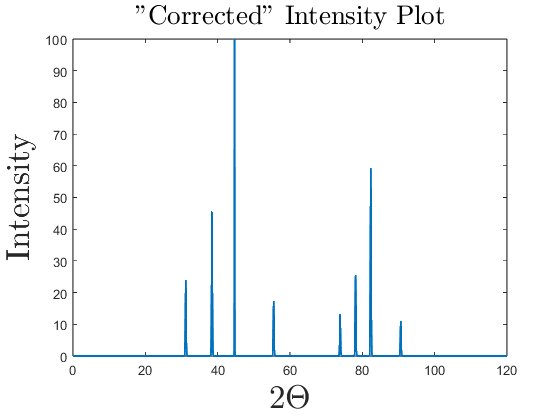
\includegraphics[scale = 0.6]{correctedintensity.png}
    \end{center}
    While this plot is expected to be more realistic compared to our first plot, it is still an extremely rough estimate given the plots for atomic form factors. That is to say it is an $\mathcal{O}(1)$ or "zeroth" order approximation.
\end{enumerate}

\end{document}
